\documentclass[aspectratio=169]{beamer}

\usepackage[utf8]{inputenc}
\usepackage[T1]{fontenc}
\usepackage{amsmath,amssymb}
\usepackage{booktabs}
\usepackage{graphicx}

\usetheme{Madrid}
\usecolortheme{default}

\definecolor{BootcampBlue}{HTML}{1A3C68}
\definecolor{BootcampGold}{HTML}{C69214}
\definecolor{BootcampRed}{HTML}{9A1B1E}
\definecolor{BootcampGreen}{HTML}{2F7D32}

\setbeamercolor{structure}{fg=BootcampBlue}
\setbeamercolor{frametitle}{fg=white,bg=BootcampBlue}
\setbeamercolor{title}{fg=white,bg=BootcampBlue}
\setbeamercolor{block title}{fg=white,bg=BootcampBlue}
\setbeamercolor{block body}{fg=black,bg=BootcampBlue!6}
\setbeamercolor{alerted text}{fg=BootcampRed}

\newenvironment{resultblock}[1]{%
  \setbeamercolor{block title}{fg=black,bg=BootcampGold}%
  \setbeamercolor{block body}{fg=black,bg=BootcampGold!10}%
  \begin{block}{#1}}{\end{block}}

\newcommand{\R}{\mathbb{R}}
\newcommand{\E}{\mathbb{E}}
\newcommand{\Var}{\operatorname{Var}}
\newcommand{\diag}{\operatorname{diag}}
\newcommand{\dd}{\,\mathrm{d}}

\title[Session 2 -- Calculus and ODE]{Summer Bootcamp\\Session 2 -- Calculus and ODE}
\subtitle{Differentiation, integration, Taylor expansion, and financial dynamics}
\author{Nathan Sauldubois}
\institute{NYU Finance and Risk Engineering}
\date{August 2026}

\AtBeginSection[]{
\begin{frame}{Section Roadmap}
  \small
  \tableofcontents[currentsection,sectionstyle=show/hide,
    subsectionstyle=show/show/hide]
\end{frame}
}

\begin{document}

\begin{frame}
  \titlepage
\end{frame}

\begin{frame}{Session Roadmap}
\begin{block}{Learning goals}
By the end of the session, students should be able to:
\begin{itemize}
  \item compare approximation errors using Landau notation;
  \item compute derivatives, gradients, Jacobians, and Hessians;
  \item use Taylor expansion for approximation and local analysis;
  \item manipulate integrals, substitutions, and differentiation under the integral sign;
  \item solve scalar and multidimensional linear ODEs;
  \item connect ODEs to risk-free growth, discounting, and Vasicek mean reversion.
\end{itemize}
\end{block}
\end{frame}

\section{Landau Notation and Approximation}

\begin{frame}{Landau Notation Compares Scales}
Let $f$ and $g$ be defined near $a$, with $g(x)\neq0$ for $x\neq a$.
\begin{block}{Big $O$: bounded relative size}
We write $f(x)=O(g(x))$ as $x\to a$ if there exist $C,\delta>0$ such that
\[
0<|x-a|<\delta
\quad\Longrightarrow\quad
|f(x)|\leq C|g(x)|.
\]
\end{block}
\pause
\begin{block}{Small $o$: negligible relative size}
We write $f(x)=o(g(x))$ as $x\to a$ if
\[
\frac{f(x)}{g(x)}\longrightarrow0.
\]
\end{block}
Thus $O(g)$ means ``at most the scale of $g$'', whereas $o(g)$ means
``strictly smaller than the scale of $g$''.
\end{frame}

\begin{frame}{Examples in One Dimension}
As $h\to0$, determine the correct $O$ or $o$ relation for each expression:
\[
h^3\ \text{versus }h^2,
\qquad 3h^2-h^3\ \text{versus }h^2,
\qquad \sin h-h\ \text{versus }h^2.
\]
\pause
The answers are
\[
h^3=o(h^2),
\qquad
3h^2-h^3=O(h^2),
\qquad
\sin h=h+O(h^3).
\]
\pause
Indeed,
\[
\frac{h^3}{h^2}=h\to0,
\qquad
\left|\frac{3h^2-h^3}{h^2}\right|=|3-h|\leq4
\]
for $|h|<1$.
\pause
\begin{alertblock}{The distinction matters}
$h^2=O(h^2)$, but $h^2\neq o(h^2)$ because the ratio equals $1$.
Moreover, $o(g)\subset O(g)$ near the limit point.
\end{alertblock}
\end{frame}

\begin{frame}{Landau Notation Encodes Local Expansions}
As $h\to0$,
\[
e^h=1+h+\frac{h^2}{2}+O(h^3),
\qquad
\log(1+h)=h-\frac{h^2}{2}+o(h^2).
\]
\pause
For a differentiable function at $a$,
\[
f(a+h)=f(a)+f'(a)h+o(|h|).
\]
The remainder is negligible compared with the linear term's natural scale.
\pause
\begin{exampleblock}{Example}
Use $\sqrt{1+h}=1+\tfrac12h+O(h^2)$ to expand $\sqrt{4+x}$ as $x\to0$.
\pause
\[
\sqrt{4+x}=2\sqrt{1+\frac{x}{4}}
=2+\frac{x}{4}+O(x^2)
\qquad (x\to0).
\]
\end{exampleblock}
\end{frame}

\begin{frame}{The Same Definitions Work in $\R^d$}
Let $F:\R^d\to\R^m$ and let $G:\R^d\to[0,\infty)$.
Using any norm, as $h\to0$ in $\R^d$,
\[
F(h)=O(G(h))
\iff
\|F(h)\|\leq C G(h)\quad\text{near }0,
\]
\[
F(h)=o(G(h))
\iff
\frac{\|F(h)\|}{G(h)}\longrightarrow0.
\]
\pause
\begin{exampleblock}{Polynomial examples}
For $h=(h_1,h_2)\to0$, compare $h_1h_2$ and $h_1^2h_2$ with
$\|h\|^2$.
\pause
\[
h_1h_2=O(\|h\|^2),
\qquad
h_1^2h_2=o(\|h\|^2).
\]
Indeed, $|h_1h_2|\leq\tfrac12\|h\|^2$ and
$|h_1^2h_2|\leq\|h\|^3=o(\|h\|^2)$.
\end{exampleblock}
\end{frame}

\section{One-Dimensional Differentiation}

\begin{frame}{Derivative: Definition and Meaning}
\begin{block}{Definition}
For a function $f:\R\to\R$,
\[
f'(x)=\lim_{h\to 0}\frac{f(x+h)-f(x)}{h},
\]
when the limit exists.
\end{block}
\pause
\begin{itemize}
  \item Instantaneous rate of change.
  \item Slope of the tangent line at $(x,f(x))$.
  \item Local linear approximation:
  \[
  f(x+h)\approx f(x)+f'(x)h.
  \]
\end{itemize}
\end{frame}

\begin{frame}{$C^1$ Regularity in One Dimension}
Let $I\subset\R$ be an open interval and let $f:I\to\R$.
\begin{block}{Definition}
$f\in C^1(I)$ if $f$ is differentiable at every point of $I$ and
$f':I\to\R$ is continuous.
\end{block}
\pause
Differentiability alone does not imply $C^1$ regularity: continuity of the
derivative is an additional requirement.
\begin{exampleblock}{Quick check}
$x\mapsto e^x$ and $x\mapsto|x|^3$ are in $C^1(\R)$, whereas
$x\mapsto|x|$ is not differentiable at $0$.
\end{exampleblock}
\end{frame}

\begin{frame}{Differentiation Rules}
\small
For differentiable functions $f,g$ and constants $a,b$:
\[
(af+bg)'=af'+bg',
\]
\[
(fg)'=f'g+fg',
\qquad
\left(\frac{f}{g}\right)'=\frac{f'g-fg'}{g^2}.
\]
\pause
\begin{resultblock}{Result -- Chain rule}
If $F(x)=f(g(x))$, then
\[
\boxed{F'(x)=f'(g(x))g'(x).}
\]
\end{resultblock}
\pause
\begin{exampleblock}{Example}
Compute the derivative of $x\mapsto(2x+1)^4$.
\pause
\[
\frac{\dd}{\dd x}(2x+1)^4=4(2x+1)^3\cdot 2=8(2x+1)^3.
\]
\end{exampleblock}
\end{frame}

\begin{frame}{Classic Derivatives}
\begin{center}
\begin{tabular}{@{}ll@{}}
\toprule
Function & Derivative \\
\midrule
$x^n$ & $nx^{n-1}$ \\
$e^x$ & $e^x$ \\
$\log x$ & $1/x$, for $x>0$ \\
$\sin x$ & $\cos x$ \\
$\cos x$ & $-\sin x$ \\
\bottomrule
\end{tabular}
\end{center}
\end{frame}

\begin{frame}{One-Dimensional Derivative Toolkit}
For differentiable $f,g$ and constant $a$:
\[
\begin{aligned}
(fg)'&=f'g+fg',
&\left(\frac fg\right)'&=\frac{f'g-fg'}{g^2},\\
(f\circ g)'&=(f'\circ g)g',
&(g^a)'&=ag^{a-1}g',\\
(e^{g})'&=e^g g',
&(\log g)'&=\frac{g'}{g}.
\end{aligned}
\]
\end{frame}

\begin{frame}{Rolle's Theorem}
\begin{columns}[T,onlytextwidth]
\begin{column}{0.48\textwidth}
\begin{resultblock}{Result}
If $f$ is continuous on $[a,b]$, differentiable on $(a,b)$, and
$f(a)=f(b)$, then there exists $c\in(a,b)$ such that
\[
\boxed{f'(c)=0.}
\]
\end{resultblock}
\end{column}
\begin{column}{0.50\textwidth}
\centering
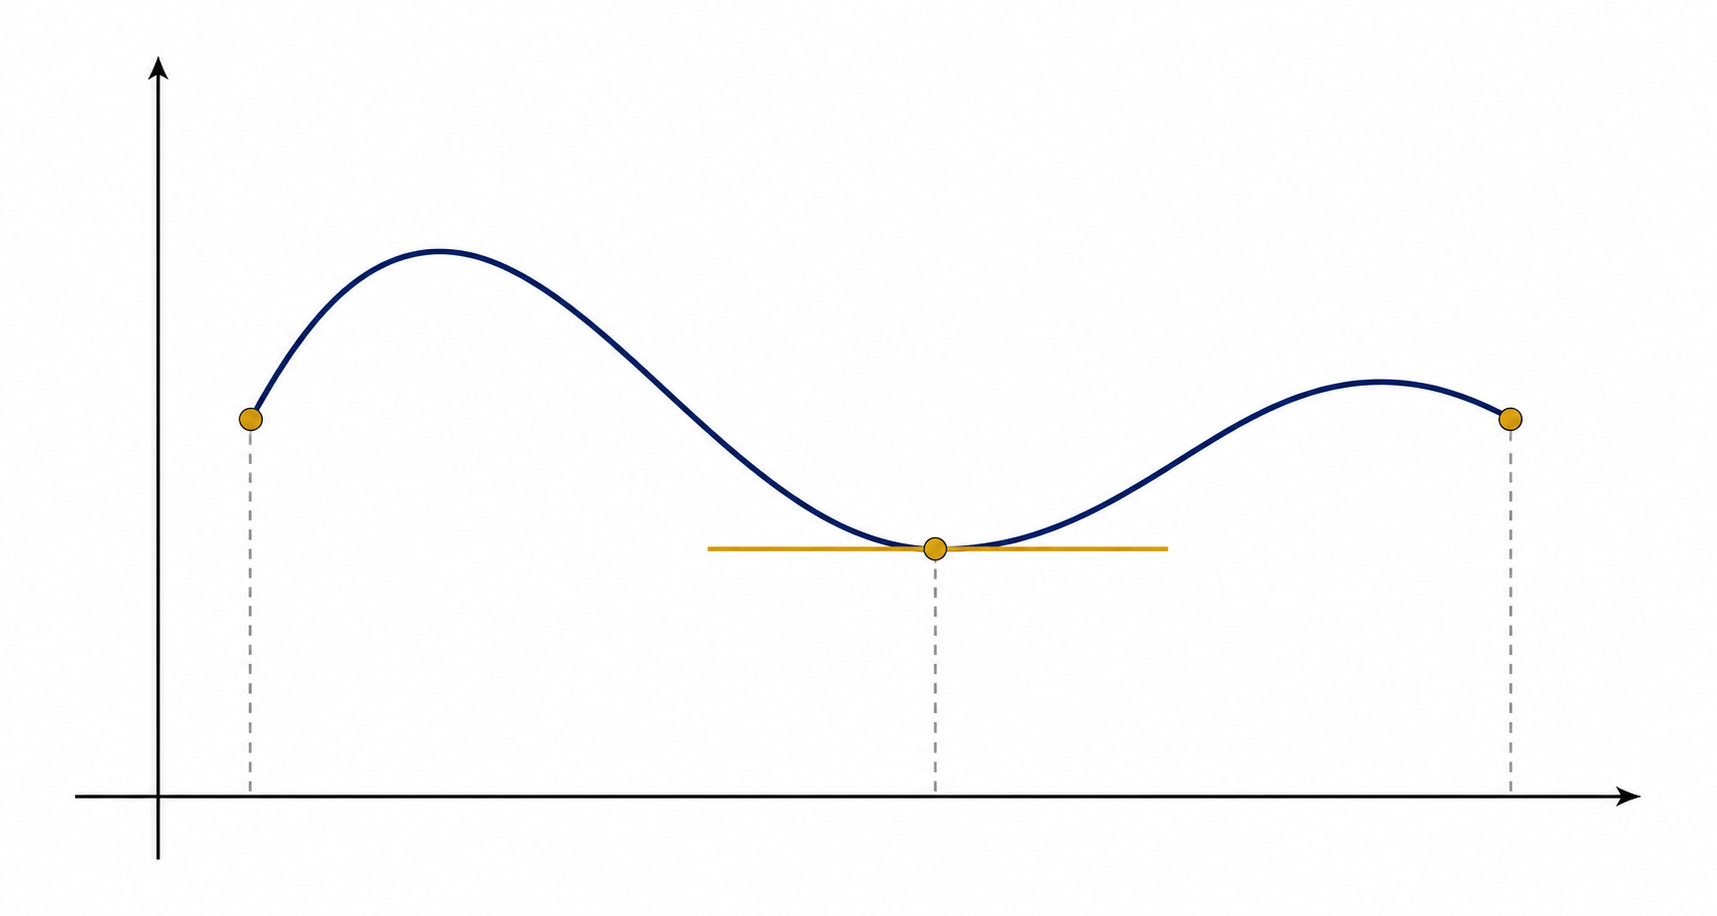
\includegraphics[width=\linewidth]{assets/rolle-theorem.png}
\[
f(a)=f(b),\qquad f'(c)=0.
\]
\end{column}
\end{columns}
\pause
For $f(x)=x^2-4x$ on $[0,4]$, find a point guaranteed by Rolle's theorem.
\pause
Since $f'(x)=2x-4$, Rolle's point is $c=2$.
\end{frame}

\begin{frame}{Mean Value Theorem}
\begin{resultblock}{Result -- Mean value theorem}
If $f$ is continuous on $[a,b]$ and differentiable on $(a,b)$, then for some
$c\in(a,b)$,
\[
\boxed{f(b)-f(a)=f'(c)(b-a).}
\]
\end{resultblock}
\end{frame}

\begin{frame}{The Sign of the Derivative Controls Monotonicity}
\begin{resultblock}{Consequence -- Monotonicity criteria}
Let $f$ be differentiable on an interval $I$.
\[
\boxed{
\begin{array}{rcl}
f'(x)\geq0\ \text{on }I &\Longrightarrow& f\text{ is nondecreasing},\\[2pt]
f'(x)>0\ \text{on }I &\Longrightarrow& f\text{ is strictly increasing},\\[2pt]
f'(x)\leq0\ \text{on }I &\Longrightarrow& f\text{ is nonincreasing},\\[2pt]
f'(x)=0\ \text{on }I &\Longrightarrow& f\text{ is constant}.
\end{array}}
\]
\end{resultblock}

Indeed, for $x<y$, the mean value theorem gives a point $c\in(x,y)$ such that
\[
f(y)-f(x)=f'(c)(y-x).
\]
Since $y-x>0$, the sign of the increment is determined by the sign of $f'(c)$.
\end{frame}

\begin{frame}{A Derivative Bound Controls All Increments}
\begin{resultblock}{Consequence -- Lipschitz estimate}
If $|f'(x)|\leq L$ on an interval $I$, then for every $x,y\in I$,
\[
\boxed{|f(y)-f(x)|\leq L|y-x|.}
\]
Thus $f$ is $L$-Lipschitz continuous on $I$.
\end{resultblock}

\pause
\begin{resultblock}{Consequence -- Uniqueness from strict monotonicity}
If $f'(x)>0$ everywhere on $I$, or $f'(x)<0$ everywhere on $I$, then $f$ is
one-to-one. In particular,
\[
\boxed{f(x)=0\text{ has at most one solution in }I.}
\]
\end{resultblock}

These conclusions are global even though the derivative is local information.
\end{frame}

\section{Multivariate Calculus}

\begin{frame}{Partial Derivatives and Gradient}
For $f:\R^n\to\R$, the partial derivative with respect to $x_i$ is
\[
\partial_{x_i}f(x)
=
\lim_{h\to 0}
\frac{f(x_1,\ldots,x_i+h,\ldots,x_n)-f(x)}{h}.
\]
\pause
The gradient is
\[
\nabla f(x)=
\begin{pmatrix}
\partial_{x_1}f(x)\\
\vdots\\
\partial_{x_n}f(x)
\end{pmatrix}.
\]
\pause
\begin{block}{Directional derivative}
For $\|u\|=1$,
\[
D_uf(x)=\nabla f(x)^\top u.
\]
The gradient points toward steepest ascent.
\end{block}
\end{frame}

\begin{frame}{The Differential Is a Linear Map}
We say that $g:\R^n\to\R^m$ is differentiable at $x$ if there exists a
\emph{linear map}
\[
Dg(x):\R^n\longrightarrow\R^m.
\]
such that
\[
g(x+h)=g(x)+Dg(x)h+o(\|h\|).
\]
\pause
Linearity means that, for increments $h,k$ and scalars $\alpha,\beta$,
\[
\boxed{Dg(x)(\alpha h+\beta k)
=\alpha Dg(x)h+\beta Dg(x)k.}
\]
\begin{alertblock}{Do not confuse the two maps}
$g$ may be nonlinear. Its differential $h\mapsto Dg(x)h$ is linear in the
increment $h$ once the base point $x$ is fixed.
\end{alertblock}
\end{frame}

\begin{frame}{Differentiability in Several Variables}
The linear map $Dg(x)$ is the best first-order approximation of $g$ at $x$:
\[
g(x+h)=g(x)+Dg(x)h+r(h),
\qquad \frac{\|r(h)\|}{\|h\|}\to0.
\]
\pause
In coordinates, the matrix of $Dg(x)$ is the Jacobian $J_g(x)$:
\[
Dg(x)h=J_g(x)h.
\]
For $f:\R^n\to\R$, this becomes
\[
f(x+h)=f(x)+\nabla f(x)^\top h+o(\|h\|).
\]
\begin{block}{Sufficient condition}
Continuous first-order partial derivatives near $x$ imply differentiability.
\end{block}
\end{frame}

\begin{frame}{$C^1$ Regularity in Several Dimensions}
Let $U\subset\R^n$ be open and let $g:U\to\R^m$.
\begin{block}{Definition}
$g\in C^1(U;\R^m)$ if $g$ is differentiable on $U$ and
\[
x\longmapsto Dg(x)\in\mathcal L(\R^n,\R^m)
\]
is continuous.
\end{block}
\pause
Equivalently, all first-order partial derivatives exist and are continuous:
\[
\partial_{x_j}g_i\in C^0(U),
\qquad 1\leq i\leq m,\quad 1\leq j\leq n.
\]
Thus $g\in C^1$ exactly when its Jacobian $J_g(x)$ varies continuously with
$x$.
\end{frame}

\begin{frame}{Exercise 1: Compute a Gradient with Partial Derivatives}
For
\[
f(x,y)=x^2+3xy+2y^2,
\qquad
\nabla f(x,y)=\begin{pmatrix}\phantom{\partial_x f}\\[2mm]\phantom{\partial_y f}\end{pmatrix}.
\]
\pause
Compute one coordinate at a time:
\[
\partial_x f(x,y)=2x+3y,
\qquad
\partial_y f(x,y)=3x+4y.
\]
Therefore
\[
\boxed{\nabla f(x,y)=\begin{pmatrix}2x+3y\\3x+4y\end{pmatrix}.}
\]
\end{frame}

\begin{frame}{Vector-Valued Functions and Jacobian}
For a map $g:\R^n\to\R^m$,
\[
g(x)=
\begin{pmatrix}
g_1(x)\\
\vdots\\
g_m(x)
\end{pmatrix},
\]
the Jacobian matrix is
\[
J_g(x)=
\begin{pmatrix}
\partial_{x_1}g_1(x)&\cdots&\partial_{x_n}g_1(x)\\
\vdots&\ddots&\vdots\\
\partial_{x_1}g_m(x)&\cdots&\partial_{x_n}g_m(x)
\end{pmatrix}.
\]
\pause
\begin{block}{Interpretation}
$J_g(x)$ is the best linear approximation of $g$ near $x$.
\end{block}
\end{frame}

\begin{frame}{Jacobian Example}
Let
\[
\Phi(u,v)=(ue^v,\ u^2+v).
\]
Compute
\[
J_\Phi(u,v)=\underline{\hspace{3.2cm}},
\qquad
\det J_\Phi(u,v)=\underline{\hspace{2.2cm}}.
\]
\pause
Then
\[
J_\Phi(u,v)=
\begin{pmatrix}
\partial_u(ue^v)&\partial_v(ue^v)\\
\partial_u(u^2+v)&\partial_v(u^2+v)
\end{pmatrix}
=
\begin{pmatrix}
e^v&ue^v\\
2u&1
\end{pmatrix}.
\]
\pause
The determinant is
\[
\det J_\Phi(u,v)=e^v(1-2u^2).
\]
\end{frame}

\begin{frame}{Exercise 2: Derive the Multivariate Chain Rule}
\footnotesize
\setlength{\abovedisplayskip}{4pt}
\setlength{\belowdisplayskip}{4pt}
Let $g:\R^n\to\R^m$ and $f:\R^m\to\R$.
\begin{exampleblock}{Task}
Find the first-order expansion of
\[
(f\circ g)(x+h)-(f\circ g)(x)
\]
and deduce $\nabla(f\circ g)(x)$.
\end{exampleblock}
\pause
\textbf{Step 1.} First expand the inner function:
\[
g(x+h)=g(x)+J_g(x)h+o(\|h\|).
\]
\pause
\textbf{Step 2.} Set $k=J_g(x)h+o(\|h\|)$ and expand the outer function:
\[
f(g(x)+k)=f(g(x))+\nabla f(g(x))^\top k+o(\|k\|).
\]
\pause
Combining the two expansions gives
\[
f(g(x+h))-f(g(x))
=\nabla f(g(x))^\top J_g(x)h+o(\|h\|).
\]
Therefore
\[
\boxed{\nabla(f\circ g)(x)=J_g(x)^\top\nabla f(g(x)).}
\]
\end{frame}

\begin{frame}{The Same Chain Rule in Partial Derivatives}
Write $g=(g_1,\ldots,g_m)$. For every input coordinate $x_j$,
\[
\boxed{
\partial_{x_j}(f\circ g)(x)
=\sum_{i=1}^m
\partial_{y_i}f(g(x))\,\partial_{x_j}g_i(x).}
\]
\pause
This is exactly the $j$-th component of
\[
J_g(x)^\top\nabla f(g(x)).
\]
Thus the increment calculation and the coordinate calculation give the same
formula: the Jacobian transports the first-order variation through the
composition.
\end{frame}

\begin{frame}{Scalar Product: Two Ways to Find the Differential}
Let $p(x,y)=x^\top y$ for $x,y\in\R^n$.
\pause
Coordinatewise,
\[
\partial_{x_i}p=y_i,
\qquad
\partial_{y_i}p=x_i,
\qquad
\boxed{\nabla p(x,y)=\begin{pmatrix}y\\x\end{pmatrix}.}
\]
\pause
For increments $(h,k)$,
\[
p(x+h,y+k)-p(x,y)
=y^\top h+x^\top k+h^\top k.
\]
The linear part is therefore
\[
\boxed{Dp(x,y)(h,k)=y^\top h+x^\top k.}
\]
\end{frame}

\begin{frame}{Quadratic Form: Two Ways to Find the Gradient}
Let $q(x)=x^\top Ax$, where $A\in\R^{n\times n}$.
\pause
Using partial derivatives,
\[
\partial_{x_i}q(x)
=\sum_j A_{ij}x_j+\sum_j A_{ji}x_j,
\qquad
\boxed{\nabla q(x)=(A+A^\top)x.}
\]
\pause
Using an increment $h$,
\[
q(x+h)-q(x)
=x^\top Ah+h^\top Ax+h^\top Ah.
\]
Hence
\[
Dq(x)h=((A+A^\top)x)^\top h.
\]
If $A$ is symmetric, $\nabla q(x)=2Ax$.
\end{frame}

\section{Implicit and Inverse Function Theorems}

\begin{frame}{Implicit Function Theorem}
\begin{resultblock}{Result -- Implicit function theorem}
Suppose $F(x_0,y_0)=0$ and
\[
\partial_yF(x_0,y_0)\neq0.
\]
If $F$ is continuously differentiable, then locally the equation $F(x,y)=0$
defines a unique differentiable function $y=\varphi(x)$.
\pause
Differentiating $F(x,\varphi(x))=0$ gives
\[
\boxed{\varphi'(x)=-\frac{\partial_xF(x,\varphi(x))}
{\partial_yF(x,\varphi(x))}}.
\]
\end{resultblock}
\end{frame}

\begin{frame}{Implicit Differentiation on the Unit Circle}
For $F(x,y)=x^2+y^2-1$, find $\dd y/\dd x$ wherever the curve can be
written locally as $y=\varphi(x)$.
\pause
Whenever $y\neq0$,
\[
\frac{\dd y}{\dd x}=-\frac{2x}{2y}=-\frac{x}{y}.
\]
At $(1,0)$ the condition fails: the tangent is vertical.
\end{frame}

\begin{frame}{The Inverse Problem Is to Solve $g(x)=y$}
Given a target $y\in\R^n$, we seek $x$ such that
\[
\boxed{g(x)=y.}
\]
If $g:\R^n\to\R^n$ is continuously differentiable and $J_g(x_0)$ is
invertible, then nearby targets have a unique local solution
$x=g^{-1}(y)$, with
\[
J_{g^{-1}}(g(x_0))=J_g(x_0)^{-1}.
\]
\begin{block}{Geometric meaning}
An invertible Jacobian means that the local linear approximation neither
flattens nor loses a direction.
\end{block}
\end{frame}

\begin{frame}{Newton Solves the Linearized Equation}
Set $F(x)=g(x)-y$. Starting from $x_k$, linearize:
\[
F(x_k+s)\approx F(x_k)+J_g(x_k)s.
\]
Impose $F(x_k)+J_g(x_k)s_k=0$:
\[
\boxed{J_g(x_k)s_k=y-g(x_k)},
\qquad
\boxed{x_{k+1}=x_k+s_k}.
\]
\pause
Stop when, for chosen tolerances,
\[
\|g(x_k)-y\|\leq\varepsilon_F
\quad\text{or}\quad
\|s_k\|\leq\varepsilon_x(1+\|x_k\|).
\]
\begin{alertblock}{Numerical practice}
Solve for $s_k$; never form $J_g(x_k)^{-1}$ explicitly. Newton is fast near a
solution but may fail from a poor initial guess or a nearly singular Jacobian.
\end{alertblock}
\end{frame}

\begin{frame}{In One Dimension: Bisection or Newton?}
For continuous $F:[a,b]\to\R$ with $F(a)F(b)<0$, bisection repeats:
\begin{enumerate}
  \item compute the midpoint $m=(a+b)/2$;
  \item if $F(a)F(m)\leq0$, replace $b$ by $m$;
  \item otherwise, replace $a$ by $m$;
  \item stop when the interval or residual is sufficiently small.
\end{enumerate}
After $k$ steps,
\[
|x_k-x^\star|\leq\frac{b-a}{2^{k+1}}.
\]
\begin{center}
\begin{tabular}{@{}lll@{}}
\toprule
Method & Main advantage & Main drawback\\
\midrule
Bisection & guaranteed, derivative-free & linear and relatively slow\\
Newton & quadratic convergence locally & needs $F'$ and a good initial guess\\
\bottomrule
\end{tabular}
\end{center}
\begin{block}{Common strategy}
Bracket first with bisection, then switch to Newton near the root.
\end{block}
\end{frame}

\begin{frame}{Implied Volatility Is an Implicit Function}
\begin{columns}[T,onlytextwidth]
\begin{column}{0.70\textwidth}
For a call with spot $S$, strike $K$, maturity $T$, and constant rate $r$,
\[
C_{\mathrm{BS}}(S,K,T,r,\sigma)
=S\Phi(d_1)-Ke^{-rT}\Phi(d_2),
\]
\[
d_1=\frac{\log(S/K)+(r+\tfrac12\sigma^2)T}{\sigma\sqrt T},
\qquad d_2=d_1-\sigma\sqrt T.
\]
\end{column}
\begin{column}{0.27\textwidth}
\centering
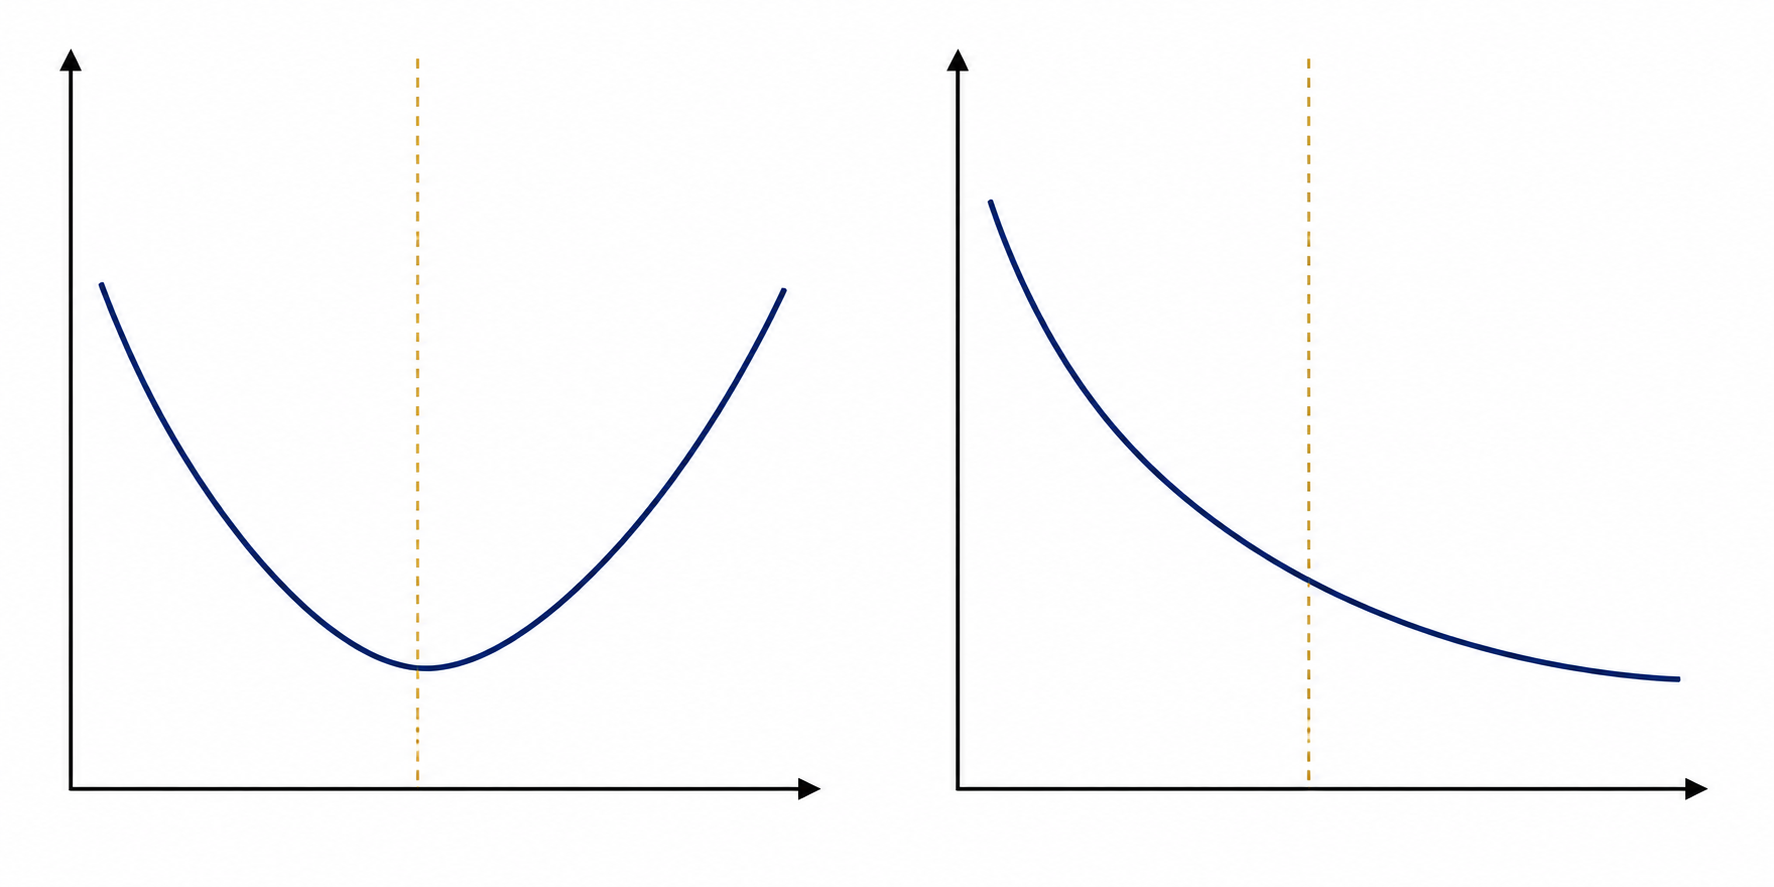
\includegraphics[width=\linewidth]{assets/vol-smile-skew.png}

\scriptsize Smile and skew across strikes.
\end{column}
\end{columns}
\pause
Define
\[
F(K,T,\sigma)=C_{\mathrm{BS}}(S,K,T,r,\sigma)-C^{\mathrm{mkt}}(K,T).
\]
Implied volatility solves $F(K,T,\sigma_{\mathrm{imp}})=0$.
\begin{alertblock}{Implicit Function Theorem}
Since $\partial_\sigma F=\mathrm{Vega}>0$ for $T>0$, the theorem defines a
locally unique differentiable function $(K,T)\mapsto\sigma_{\mathrm{imp}}(K,T)$.
\end{alertblock}
\end{frame}

\section{Second Derivatives and Hessians}

\begin{frame}{Hessian Matrix}
For $f:\R^n\to\R$, the Hessian is the matrix of second derivatives:
\[
H_f(x)=
\begin{pmatrix}
\partial_{x_1x_1}^2f(x)&\cdots&\partial_{x_1x_n}^2f(x)\\
\vdots&\ddots&\vdots\\
\partial_{x_nx_1}^2f(x)&\cdots&\partial_{x_nx_n}^2f(x)
\end{pmatrix}.
\]
\pause
\begin{block}{Schwarz theorem}
If $f$ is sufficiently regular, mixed partial derivatives commute:
\[
\partial_{x_ix_j}^2f=\partial_{x_jx_i}^2f.
\]
Then $H_f$ is symmetric.
\end{block}
\end{frame}

\begin{frame}{Hessian, Convexity, and Critical Points}
\footnotesize
\begin{resultblock}{Convexity criterion}
If $f$ is twice continuously differentiable on a convex set and
\[
\boxed{H_f(x)\succeq0\quad\text{for every }x,}
\]
then $f$ is convex.
\end{resultblock}
\pause
\begin{resultblock}{Criticality condition and second-order classification}
The point $x^\star$ is critical when
\[
\boxed{\nabla f(x^\star)=0.}
\]
At such a point:
\begin{itemize}
  \item $H_f(x^\star)\succ0$ implies a strict local minimum;
  \item $H_f(x^\star)\prec0$ implies a strict local maximum;
  \item an indefinite Hessian implies a saddle point.
\end{itemize}
\end{resultblock}
\end{frame}

\begin{frame}{Hessian Example}
Let
\[
f(x,y)=x^4+2x^2y^2+y^4=(x^2+y^2)^2.
\]
Compute
\[
\nabla f(x,y)=\underline{\hspace{3cm}},
\qquad
H_f(x,y)=\underline{\hspace{3cm}}.
\]
\pause
\[
\nabla f(x,y)=
\begin{pmatrix}
4x(x^2+y^2)\\
4y(x^2+y^2)
\end{pmatrix}.
\]
\pause
\[
H_f(x,y)=
\begin{pmatrix}
12x^2+4y^2&8xy\\
8xy&4x^2+12y^2
\end{pmatrix}.
\]
\pause
This Hessian is positive semidefinite, so $f$ is convex.
\end{frame}

\begin{frame}{Hands-On Example: Least Squares}
\footnotesize
\setlength{\abovedisplayskip}{4pt}
\setlength{\belowdisplayskip}{4pt}
For
\[
L(x)=\tfrac12\|Ax-b\|^2,
\]
compute
\[
\nabla L(x)=\;?,
\qquad
H_L(x)=\;?.
\]
\pause
Since
\[
L(x)=\tfrac12(Ax-b)^\top(Ax-b),
\]
we obtain
\[
\boxed{\nabla L(x)=A^\top(Ax-b)},
\qquad
\boxed{H_L(x)=A^\top A}.
\]
\pause
With
\[
A=\begin{pmatrix}1&0\\1&1\\1&2\end{pmatrix},
\qquad b=\begin{pmatrix}1\\2\\2\end{pmatrix},
\]
find the least-squares minimizer.
\pause
The normal equations are
\[
\begin{pmatrix}3&3\\3&5\end{pmatrix}x
=\begin{pmatrix}5\\6\end{pmatrix},
\qquad
\boxed{x^\star=\begin{pmatrix}7/6\\1/2\end{pmatrix}}.
\]
Full column rank makes $A^\top A$ positive definite, so the minimizer is unique.
\end{frame}

\section{Taylor Expansion}

\begin{frame}{Taylor Expansion in One Dimension}
\begin{resultblock}{Result -- Taylor expansion at order $k$}
If $f$ is sufficiently smooth near $x$, then
\[
\boxed{
f(x+h)=f(x)+f'(x)h+\frac{1}{2}f''(x)h^2+\cdots+
\frac{1}{k!}f^{(k)}(x)h^k+R_k(h).}
\]
\end{resultblock}
\pause
\begin{block}{First and second order approximations}
\[
f(x+h)\approx f(x)+f'(x)h,
\]
\[
f(x+h)\approx f(x)+f'(x)h+\frac{1}{2}f''(x)h^2.
\]
\end{block}
\end{frame}

\begin{frame}{Taylor Examples}
Around $0$:
\[
e^x=1+x+\frac{x^2}{2}+\frac{x^3}{6}+\cdots
\]
\[
\log(1+x)=x-\frac{x^2}{2}+\frac{x^3}{3}-\cdots
\]
\[
\sin x=x-\frac{x^3}{6}+\frac{x^5}{120}-\cdots
\]
\pause
\begin{block}{Use}
Taylor expansions convert nonlinear problems into local polynomial approximations.
\end{block}
\end{frame}

\begin{frame}{Taylor Remainder and Error Control}
If $f$ is $(k+1)$ times continuously differentiable, then for some $\xi$
between $x$ and $x+h$,
\[
f(x+h)=\sum_{j=0}^k\frac{f^{(j)}(x)}{j!}h^j
+\frac{f^{(k+1)}(\xi)}{(k+1)!}h^{k+1}.
\]
\pause
Use the quadratic Taylor polynomial to approximate $e^{0.1}$ and bound the
remainder.
\pause
The result is
\[
1+0.1+\frac{0.1^2}{2}=1.105,
\qquad
|R_2|\leq\frac{e^{0.1}}{6}(0.1)^3<1.85\times10^{-4}.
\]
\begin{block}{Message}
Taylor's theorem provides both an approximation and a certified error bound.
\end{block}
\end{frame}

\begin{frame}{Multivariate Taylor Expansion}
\begin{resultblock}{Result -- Second-order multivariate expansion}
For $f:\R^n\to\R$ and small $h\in\R^n$,
\[
\boxed{
f(x+h)=f(x)+\nabla f(x)^\top h
+\frac{1}{2}h^\top H_f(x)h+o(\|h\|^2).}
\]
\end{resultblock}
\pause
\begin{block}{Interpretation}
\begin{itemize}
  \item $\nabla f(x)^\top h$ is the local linear effect.
  \item $h^\top H_f(x)h$ is the local curvature effect.
  \item The Hessian controls second-order behavior.
\end{itemize}
\end{block}
\end{frame}

\begin{frame}{Taylor and Local Optimization}
Near a critical point $x^\star$ with $\nabla f(x^\star)=0$,
\[
f(x^\star+h)\approx f(x^\star)+\frac{1}{2}h^\top H_f(x^\star)h.
\]
\pause
\begin{itemize}
  \item If $H_f(x^\star)$ is positive definite, $x^\star$ is a local minimum.
  \item If $H_f(x^\star)$ is negative definite, $x^\star$ is a local maximum.
  \item If $H_f(x^\star)$ is indefinite, $x^\star$ is a saddle point.
\end{itemize}
\pause
\begin{block}{Bridge to Session 3}
Optimization is built on gradients, Hessians, and Taylor approximations.
\end{block}
\end{frame}

\section{Integration}

\begin{frame}{Integrals and the Fundamental Theorem}
\small
The integral $\int_a^b f(x)\dd x$ measures accumulated quantity over an interval.
\pause
\begin{resultblock}{Result -- Fundamental theorem of calculus}
If $F'(x)=f(x)$, then
\[
\boxed{\int_a^b f(x)\dd x=F(b)-F(a).}
\]
\end{resultblock}
\pause
\begin{resultblock}{Corollary -- Differentiating the upper bound}
If $f$ is continuous and
\[
G(x)=\int_a^x f(t)\dd t,
\qquad
\boxed{G'(x)=\frac{\dd}{\dd x}\int_a^x f(t)\dd t=f(x).}
\]
\end{resultblock}
\end{frame}

\begin{frame}{Example: Integrating Exponential Growth}
\begin{exampleblock}{Example}
Compute $\displaystyle\int_0^T e^{rt}\dd t$ for $r\in\R$.
\pause
\[
\int_0^T e^{rt}\dd t=
\begin{cases}
\dfrac{e^{rT}-1}{r},& r\neq 0,\\
T,& r=0.
\end{cases}
\]
\end{exampleblock}
\pause
\begin{block}{Why the case $r=0$ is consistent}
The limit of $(e^{rT}-1)/r$ as $r\to0$ equals $T$.
\end{block}
\end{frame}

\begin{frame}{Change of Variables}
\footnotesize
\begin{resultblock}{Result -- One-dimensional change of variables}
If $u=\phi(x)$ and $\phi$ is differentiable, then
\[
\boxed{
\int_a^b f(\phi(x))\phi'(x)\dd x
=
\int_{\phi(a)}^{\phi(b)} f(u)\dd u.}
\]
\end{resultblock}
\pause
\begin{exampleblock}{Example}
\[
\int_0^1 \frac{1}{\sqrt{1-x^2}}\dd x.
\]
Choose a substitution and evaluate the integral.
\textbf{Hint:} set $x=\sin u$ so that $1-x^2=\cos^2u$.
\pause
Use $x=\sin u$, so $\dd x=\cos u\dd u$ and $u:0\to \pi/2$:
\[
\int_0^{\pi/2}1\dd u=\frac{\pi}{2}.
\]
\end{exampleblock}
\end{frame}

\begin{frame}{Change of Variables in $\R^n$}
\small
Let $\Phi:U\to V$ be a $C^1$ diffeomorphism between open subsets of
$\R^n$. Then
\begin{resultblock}{Result -- Multidimensional change of variables}
\[
\boxed{
\int_V f(y)\dd y
=\int_U f(\Phi(x))\left|\det J_\Phi(x)\right|\dd x.}
\]
More generally, for $D\subset U$,
\[
\boxed{
\int_{\Phi(D)}f(y)\dd y
=\int_D f(\Phi(x))\left|\det J_\Phi(x)\right|\dd x.}
\]
\end{resultblock}
\pause
$|\det J_\Phi(x)|$ is the local factor by which $\Phi$ scales
$n$-dimensional volume.
\end{frame}

\begin{frame}{Polar Coordinates}
For $\Phi(r,\theta)=(r\cos\theta,r\sin\theta)$,
\[
|\det J_\Phi(r,\theta)|=r.
\]
Evaluate the following integral over the disk of radius $R$:
\[
\iint_{x^2+y^2\le R^2}(x^2+y^2)\dd x\dd y.
\]
\pause
Using polar coordinates,
\[
\iint_{x^2+y^2\le R^2}(x^2+y^2)\dd x\dd y
=\int_0^{2\pi}\int_0^Rr^3\dd r\dd\theta
=\boxed{\frac{\pi R^4}{2}}.
\]
\end{frame}

\begin{frame}{Integration by Parts}
\small
\setlength{\abovedisplayskip}{4pt}
\setlength{\belowdisplayskip}{4pt}
\begin{resultblock}{Result -- Integration by parts}
For continuously differentiable functions $u$ and $v$,
\[
\boxed{
\int_a^b u(x)v'(x)\dd x
=
\left[u(x)v(x)\right]_a^b-\int_a^b u'(x)v(x)\dd x.}
\]
\end{resultblock}
\pause
\begin{exampleblock}{Example}
Evaluate $\displaystyle\int_0^T te^{-at}\dd t$ by parts, for $a>0$.
\pause
Choose the factor to differentiate and the factor to integrate:
\[
u(t)=t,
\qquad \dd u=\dd t,
\qquad
\dd v=e^{-at}\dd t,
\qquad v(t)=-\frac1a e^{-at}.
\]
\pause
Therefore
\[
\int_0^Tte^{-at}\dd t
=\left[-\frac{t}{a}e^{-at}\right]_0^T
+\frac1a\int_0^Te^{-at}\dd t
=\boxed{\frac{1-e^{-aT}(1+aT)}{a^2}}.
\]
\end{exampleblock}
\end{frame}

\begin{frame}{Leibniz Rule}
\begin{resultblock}{Result -- Leibniz rule}
Let
\[
F(\theta)=\int_{a(\theta)}^{b(\theta)} f(x,\theta)\dd x.
\]
\pause
Then
\[
\boxed{
F'(\theta)
=f(b(\theta),\theta)b'(\theta)
-f(a(\theta),\theta)a'(\theta)
+\int_{a(\theta)}^{b(\theta)}\partial_\theta f(x,\theta)\dd x.}
\]
\end{resultblock}
\pause
\begin{block}{Finance link}
Greeks often come from differentiating prices written as expectations or integrals.
\end{block}
\end{frame}

\begin{frame}{Sensitivity of an Expectation}
Suppose
\[
P(\theta)=\E[g(X_\theta)]
=\int_\R g(x)p(x,\theta)\dd x.
\]
\pause
When the interchange is justified,
\[
\frac{\partial P}{\partial\theta}
=
\int_\R g(x)\partial_\theta p(x,\theta)\dd x.
\]
\pause
\begin{block}{Interpretation}
Differentiating under the integral sign turns pricing sensitivities into calculus problems.
\end{block}
\end{frame}

\section{Ordinary Differential Equations}

\subsection{Theoretical Results}

\begin{frame}{Ordinary Differential Equations}
An ordinary differential equation describes the time evolution of an unknown function.
\[
y'(t)=f(t,y(t)),
\qquad y(0)=y_0.
\]
\pause
\begin{itemize}
  \item The derivative gives the instantaneous direction of motion.
  \item The initial condition selects one trajectory.
  \item Financial state variables often evolve through differential equations.
\end{itemize}
\end{frame}

\begin{frame}{Existence and Uniqueness of an ODE}
\small
\begin{resultblock}{Result -- Picard--Lindelöf}
For
\[
y'(t)=f(t,y(t)),
\qquad y(t_0)=y_0,
\]
Picard--Lindelöf says:
\begin{itemize}
  \item continuity of $f$ gives local existence;
  \item local Lipschitz continuity in $y$ gives local uniqueness.
\end{itemize}
\end{resultblock}
\begin{block}{How to check the hypothesis}
Near every $(t_0,y_0)$, there are a neighborhood and $L<\infty$ such that
\[
|f(t,y_1)-f(t,y_2)|\leq L|y_1-y_2|
\]
for points in that neighborhood. A continuous $\partial_yf$ is sufficient.
\end{block}
\pause
Without the Lipschitz condition, uniqueness may fail.
\end{frame}

\subsection{General Scalar Calculations}

\begin{frame}{The Fundamental Solution Propagates Initial Data}
\begin{resultblock}{Result -- Homogeneous scalar linear ODE}
Start with the homogeneous equation
\[
y'(t)=a(t)y(t),
\qquad y(0)=y_0.
\]
Its fundamental solution is
\[
\boxed{\Phi(t,0)=\exp\left(\int_0^t a(u)\dd u\right).}
\]
\pause
It satisfies
\[
\partial_t\Phi(t,0)=a(t)\Phi(t,0),
\qquad \Phi(0,0)=1.
\]
Therefore
\[
\boxed{y(t)=\Phi(t,0)y_0.}
\]
\end{resultblock}
\end{frame}

\begin{frame}{Variation of the Constant Adds the Forcing}
Consider
\[
y'(t)=a(t)y(t)+b(t),
\qquad y(0)=y_0.
\]
Seek $y(t)=c(t)\Phi(t,0)$. Then
\[
y'=c'\Phi+c\,a(t)\Phi.
\]
\pause
Substitution gives
\[
c'(t)\Phi(t,0)=b(t),
\qquad
c(t)=y_0+\int_0^t\Phi(s,0)^{-1}b(s)\dd s.
\]
Using $\Phi(t,0)\Phi(s,0)^{-1}=\Phi(t,s)$,
\begin{resultblock}{Result -- Scalar variation-of-constants formula}
\[
\boxed{y(t)=\Phi(t,0)y_0+\int_0^t\Phi(t,s)b(s)\dd s.}
\]
\end{resultblock}
\end{frame}

\begin{frame}{Linear ODE: Exponential Growth and Decay}
Consider
\[
y'(t)=ky(t),\qquad y(0)=y_0.
\]
\pause
The solution is
\[
y(t)=y_0e^{kt}.
\]
\pause
\begin{itemize}
  \item $k>0$: exponential growth.
  \item $k<0$: exponential decay.
  \item $k=0$: constant state.
\end{itemize}
\end{frame}

\begin{frame}{Worked Linear ODE Examples}
For
\[
y'-2y=t,\qquad y(0)=1,
\]
solve by variation of the constant.
\pause
Variation of the constant gives
\[
y(t)=e^{2t}\left(1+\int_0^tse^{-2s}\dd s\right)
=\boxed{\frac54e^{2t}-\frac{1+2t}{4}}.
\]
\pause
For
\[
y'+\frac{2}{1+t}y=1+t,\qquad y(0)=1,
\]
solve with an integrating factor.
\pause
The integrating factor is $(1+t)^2$, and
\[
y(t)=\boxed{\frac{(1+t)^4+3}{4(1+t)^2}}.
\]
\end{frame}

\subsection{Linear Systems in Several Dimensions}

\begin{frame}{Multidimensional Linear ODEs}
\small
A linear system has the form
\[
\boxed{x'(t)=A(t)x(t)+g(t),\qquad x(t_0)=x_0,}
\]
with $x(t)\in\R^d$ and $A(t)\in\R^{d\times d}$.
\pause
If $A$ and $g$ are continuous, the system has a unique solution on every
compact interval where they are defined.
\begin{resultblock}{Result -- Homogeneous constant-coefficient system}
When $A$ is constant in time, $x'=Ax$ has solution
\[
\boxed{x(t)=e^{tA}x_0},
\qquad
e^{tA}=I+tA+\frac{t^2A^2}{2!}+\cdots.
\]
\end{resultblock}
For time-dependent $A(t)$, one cannot generally replace the solution by
$e^{\int_0^tA(s)\dd s}$ because matrices at different times may not commute.
\end{frame}

\begin{frame}{Diagonalization Computes the Matrix Exponential}
\begin{resultblock}{Result -- Matrix exponential by diagonalization}
If $A=PDP^{-1}$ with
$D=\diag(\lambda_1,\ldots,\lambda_d)$, then
\[
\boxed{e^{tA}=Pe^{tD}P^{-1}},
\qquad
e^{tD}=\diag(e^{\lambda_1t},\ldots,e^{\lambda_dt}).
\]
\end{resultblock}
\pause
Each eigenvalue creates one dynamical mode:
\begin{itemize}
  \item $\operatorname{Re}(\lambda)<0$: decay;
  \item $\operatorname{Re}(\lambda)>0$: growth;
  \item $\operatorname{Im}(\lambda)\neq0$: oscillation.
\end{itemize}
\begin{block}{Stability criterion}
$x=0$ is asymptotically stable when every eigenvalue of $A$ has strictly
negative real part.
\end{block}
\end{frame}

\begin{frame}{Variation of Constants in $\R^d$}
\begin{resultblock}{Result -- Multidimensional variation of constants}
For $x'(t)=Ax(t)+g(t)$ with $x(0)=x_0$,
\[
\boxed{x(t)=e^{tA}x_0+\int_0^te^{(t-s)A}g(s)\dd s.}
\]
\end{resultblock}
\pause
For constant forcing $g(t)=b$ and invertible $A$, let
$x^\star=-A^{-1}b$. Then
\[
\boxed{x(t)=x^\star+e^{tA}(x_0-x^\star).}
\]
\begin{block}{Interpretation}
The exponential propagates the initial displacement; the integral accumulates
the forcing.
\end{block}
\end{frame}

\begin{frame}{Worked Two-Dimensional Linear System}
Consider
\[
x'=\begin{pmatrix}-1&1\\0&-2\end{pmatrix}x,
\qquad x(0)=\begin{pmatrix}0\\1\end{pmatrix}.
\]
Find the solution by decomposing the initial condition into eigenvectors.
\pause
The eigenpairs are
\[
\lambda_1=-1,\ v_1=\begin{pmatrix}1\\0\end{pmatrix},
\qquad
\lambda_2=-2,\ v_2=\begin{pmatrix}-1\\1\end{pmatrix}.
\]
Since $x_0=v_1+v_2$,
\[
\boxed{x(t)=\begin{pmatrix}e^{-t}-e^{-2t}\\e^{-2t}\end{pmatrix}.}
\]
Both modes decay; $e^{-t}$ dominates in the long run.
\end{frame}

\subsection{Second-Order Equations}

\begin{frame}{Second-Order Linear ODEs}
For
\[
y''+ay'+by=0,
\]
the trial solution $e^{rt}$ gives the characteristic equation
\[
r^2+ar+b=0.
\]
\pause
Distinct roots $r_1,r_2$ give
$y=C_1e^{r_1t}+C_2e^{r_2t}$; complex roots give damped oscillations.
\medskip

For
\[
y''+3y'+2y=0,\qquad y(0)=1,\quad y'(0)=0,
\]
find the solution satisfying the two initial conditions.
\pause
the roots are $-1,-2$ and
\[
\boxed{y(t)=2e^{-t}-e^{-2t}}.
\]
\end{frame}

\begin{frame}{A Second-Order ODE Is a First-Order System}
Set $x_1=y$ and $x_2=y'$. Then
\[
y''+ay'+by=f(t)
\]
is equivalent to
\[
\boxed{
\begin{pmatrix}x_1'\\x_2'\end{pmatrix}
=\begin{pmatrix}0&1\\-b&-a\end{pmatrix}
\begin{pmatrix}x_1\\x_2\end{pmatrix}
+\begin{pmatrix}0\\f(t)\end{pmatrix}.}
\]
\pause
The characteristic roots of $r^2+ar+b=0$ are exactly the eigenvalues of the
companion matrix.
\begin{block}{Unified viewpoint}
Coupled equations and higher-order scalar equations are handled with the same
matrix tools.
\end{block}
\end{frame}

\subsection{Numerical Methods}

\begin{frame}{Explicit and Implicit Euler}
For $y'=f(t,y)$ and $t_{n+1}=t_n+h$:
\[
\boxed{y_{n+1}=y_n+h f(t_n,y_n)}
\quad\text{(explicit)},
\]
\[
\boxed{y_{n+1}=y_n+h f(t_{n+1},y_{n+1})}
\quad\text{(implicit)}.
\]
\pause
\begin{resultblock}{Result -- First-order convergence}
If $f$ is continuous in $t$, Lipschitz in $y$, and sufficiently smooth along
the exact solution, then on $[0,T]$
\[
\boxed{
\max_{0\leq n\leq N}|y(t_n)-y_n|\leq C_T h.
}
\]
Both schemes are therefore first-order convergent. For implicit Euler,
$hL<1$ is a simple sufficient condition for the step equation to have a
unique solution when $f$ is $L$-Lipschitz in $y$.
\end{resultblock}
\end{frame}

\begin{frame}{Euler Schemes for Linear Systems}
\begin{columns}[c,onlytextwidth]
\begin{column}{0.46\textwidth}
For $x'=Ax+g(t)$, explicit Euler gives
\[
\boxed{x_{n+1}=(I+hA)x_n+h g(t_n).}
\]
\pause
Implicit Euler gives the linear system
\[
\boxed{(I-hA)x_{n+1}=x_n+h g(t_{n+1}).}
\]
If $A$ is constant, implicit Euler is well defined whenever
$I-hA$ is invertible.
\end{column}
\begin{column}{0.51\textwidth}
\centering
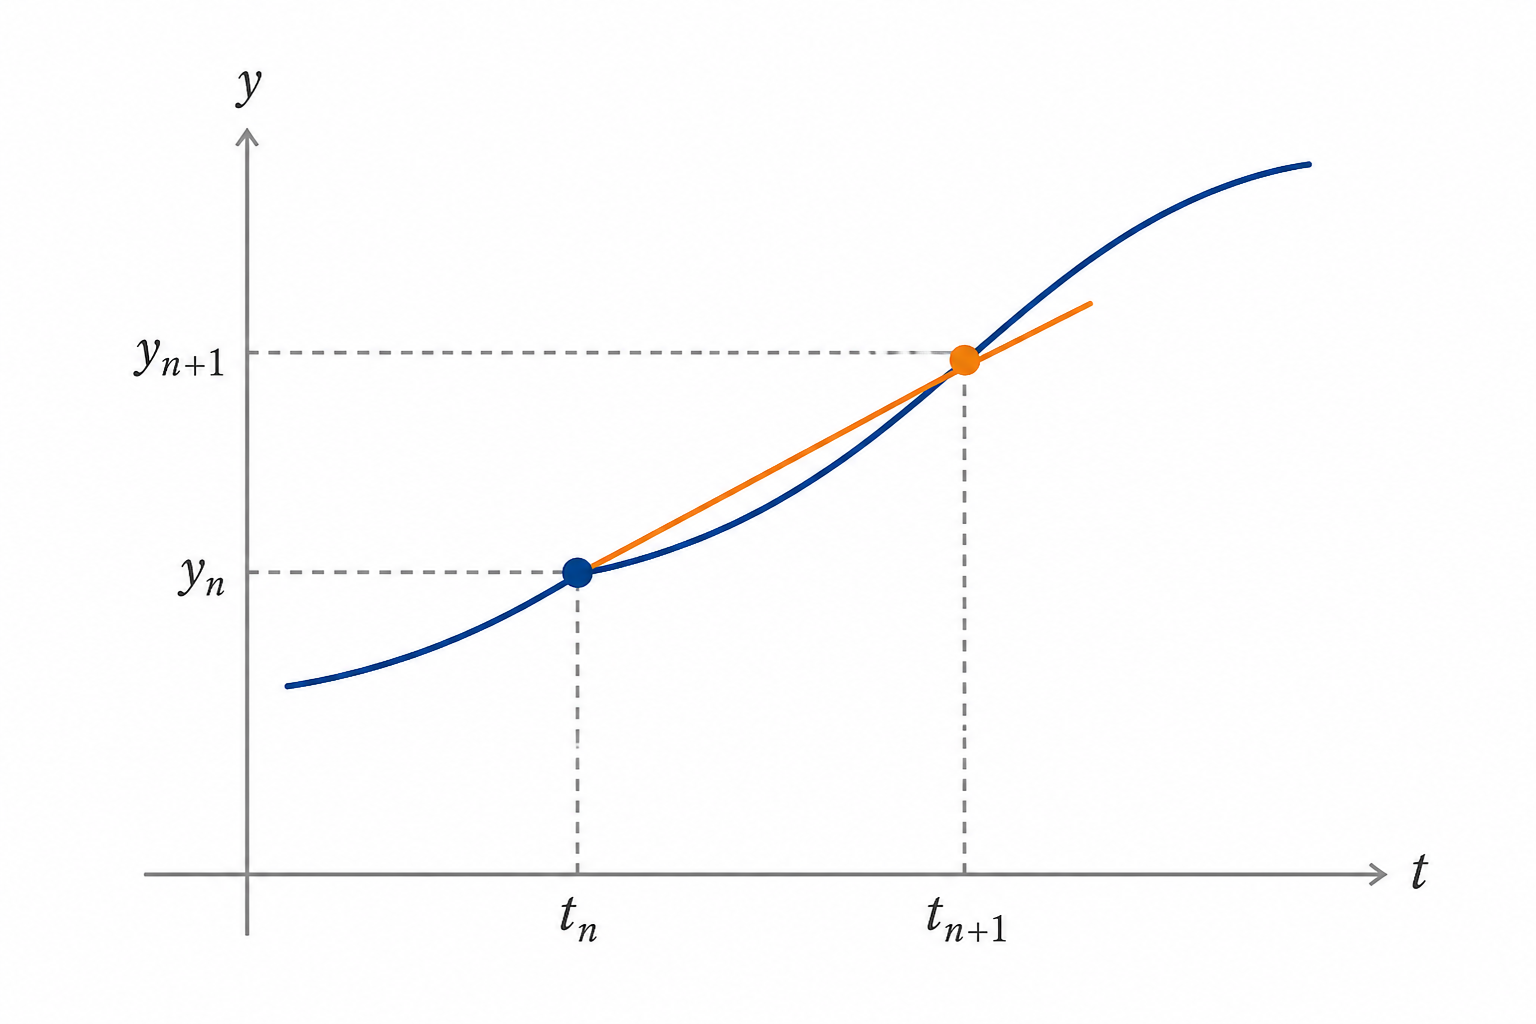
\includegraphics[width=\linewidth]{assets/euler-step-illustration.png}

\scriptsize Explicit Euler follows the tangent over one time step.
\end{column}
\end{columns}
\end{frame}

\begin{frame}{Euler Stability on $y'=\lambda y$}
Explicit Euler gives the recurrence
\[
y_{n+1}=(1+h\lambda)y_n.
\]
For real $\lambda<0$, decay requires
\[
|1+h\lambda|<1
\quad\Longleftrightarrow\quad
0<h<-\frac2\lambda.
\]
\pause
Implicit Euler gives
\[
y_{n+1}=\frac{1}{1-h\lambda}y_n,
\]
and the multiplier has modulus below one for every $h>0$ when $\lambda<0$.
Thus, for real $\lambda<0$,
\begin{resultblock}{Result -- Stability domains on the negative real axis}
\[
\text{explicit: }0<h<-2/\lambda,
\qquad
\text{implicit: every }h>0.
\]
\end{resultblock}
\end{frame}

\section{Financial Models}

\begin{frame}{Risk-Free Asset}
A risk-free bank account $B_t$ with a prescribed short-rate curve $r(t)$ satisfies
\[
\frac{\dd B_t}{\dd t}=r(t)B_t,\qquad B_0>0.
\]
\pause
The solution is
\[
B_t=B_0\exp\left(\int_0^t r(s)\dd s\right).
\]
\pause
For a constant rate $r$:
\[
B_t=B_0e^{rt}.
\]
\begin{block}{Why is this an ODE?}
Here $r(t)$ is a fixed input known as a function of time. If the short rate is
random, its dynamics require an SDE and pricing generally involves conditional
expectations.
\end{block}
\end{frame}

\begin{frame}{Continuous Discounting}
If $B_t$ is the risk-free account, the discount factor from $0$ to $T$ is
\[
D(0,T)=\frac{B_0}{B_T}
=\exp\left(-\int_0^T r(s)\dd s\right).
\]
\pause
For constant $r$,
\[
D(0,T)=e^{-rT}.
\]
\pause
\begin{block}{Pricing intuition}
The present value of a deterministic payoff $X_T$ at time $T$ is
\[
X_0=D(0,T)X_T.
\]
\end{block}
\end{frame}

\begin{frame}{Mean-Reverting ODE}
The deterministic mean-reversion equation is
\[
r'(t)=a(b-r(t)),\qquad a>0.
\]
\pause
\begin{itemize}
  \item $b$ is the long-run level.
  \item $a$ is the speed of mean reversion.
  \item If $r(t)>b$, the derivative is negative.
  \item If $r(t)<b$, the derivative is positive.
\end{itemize}
\pause
Solution:
\[
r(t)=b+(r_0-b)e^{-at}.
\]
\end{frame}

\begin{frame}{Vasicek Short-Rate Model}
The stochastic Vasicek model adds Brownian noise:
\[
\dd r_t=a(b-r_t)\dd t+\sigma\dd W_t.
\]
\pause
The conditional mean solves the deterministic mean-reversion ODE:
\[
\frac{\dd}{\dd t}\E[r_t\mid r_s]
=a\left(b-\E[r_t\mid r_s]\right).
\]
\pause
\[
\E[r_t\mid r_s]=b+(r_s-b)e^{-a(t-s)}.
\]
\end{frame}

\begin{frame}{Discounting Along the Vasicek Mean Path}
If we use the conditional mean path
$m(t)=b+(r_0-b)e^{-at}$ as the short-rate curve, then
\[
\int_0^T m(t)\dd t
=
bT+\frac{r_0-b}{a}(1-e^{-aT}).
\]
\pause
The discount factor is
\[
D(0,T)=
\exp\left(
-bT-\frac{r_0-b}{a}(1-e^{-aT})
\right).
\]
\pause
\begin{block}{Takeaway}
This computes discounting along the mean path. It is not the stochastic
Vasicek bond price, which requires an expectation of the random discount factor.
\end{block}
\end{frame}

\end{document}
